\chapter{Evaluations}\label{chap:eval}
It's very important to evaluate our work after the development. This chapter, we will evaluate our system in two aspects: data quality and system performance. Both aspect are critical to our dataset, since: without high data quality, our dataset cannot not trust by users; without high performance our approach will not be accepted by other developers and is not queryable by front-end users.

\newcommand{\round}[1]{\DTLround{#1}{#1}{4}#1}

\section{Evaluation, the rationale}

As discussed in Chapter 2, we need to evaluate the quality of the data we extracted. \cite{ochoa2006} suggest a number of quality metrics, in this project, we will use Data Completeness, Data Accuracy, User perceived data quality and Conformance to Expectation (Data fitness) to evaluate our work. The reason for choosing them is because: 

\begin{description}
	\item \textbf{Data Completeness} can reflect how complete the LinkedIn profile is. It's an important statistics we can get from LinkedIn.com as people always interest in how complete for these profiles in general. It also a hint for future research since we can quickly identify sparse data fields and intensive data fields.
	\item \textbf{Data Accuracy} is where we introduce volunteers to manually extract the data out from the HTML files and ask them to rate our results from 1 to 5. By calculating prediction precisions, recalls, f-measures (will be discussed later) and user average ratings, we can know how well our parser and our data normalisation is.
	\item \textbf{User Perceived Data Quality} is simplified version of Data Accuracy. We present our results and show the user extracted resutls, then ask user rate our result from 1 to 5. As precision, recall and f-measure are too complex for people who do not have mathematic background, simple ratings can be more user friendly.
	\item \textbf{Data fitness} is to measure how well our knowledge model and our dataset match the requirements of the upper layer user interface. In this part, we collect feedbacks from the developer of the Data Visualisation project, and the drawbacks will be presented in our future works.
\end{description}

\subsection{Data completeness}\label{subsec:datacomp}

In this section, we present the completeness of profiles in LinkedIn.com. Researchers who also interested in LinkedIn.com public profiles can use this statistics as a measure, to avoid the fields that are too sparse.

\subsubsection{Definition}

\cite{ochoa2006} defines Data completeness as: A degree of metadata contains all information required to have ideal presentation. To get it we can simple count the number of fields that contains data and divided by total number of intances:

\begin{equation}\label{eq:completeness}
	C=\frac{\sum_{i=1}^{N}F(i)}{N}
\end{equation}

In Equation~\ref{eq:completeness}, F(i) is 1 when the field has data and 0 when the field is empty. N is the total number of instances. Notice that the definition of total number of instances can be changed in later paragraph.

Table~\ref{tab:numCount} shows the total number of personal profiles, company profiles and total number of skills in all of the profiles. These numbers are base numbers that will be used to calculate the percentage in the following tables.

\begin{table}[H]
    \begin{tabular}{|c|c|}
    \hline
    Total number of public personal profiles & 13014 \\ \hline
    Total number of company profiles         & 24778 \\ \hline
    Total number of skills                   & 15917 \\ \hline
    \end{tabular}
    \caption{Total number of personal profiles, company profiles and skills}
  	\label{tab:numCount}
\end{table}

\subsubsection{Public personal profile completeness}\label{subsubsec:personProfileComp}

Many people do not fill their complete work experiences and education backgrounds into LinkedIn, therefore, in our 13014 randomly download and selected profiles, we can have an overview of the percentage of people have sections that are missing.

\begin{table}[H]
    \begin{tabular}{|c|c|c|}
    \hline
    ~                                                             & Number & Percentage(of personal profiles) \\ \hline
    Profiles that have work experiences                           & 11501  & 88.4\%                             \\ \hline
    Profiles that have education                                  & 9913   & 77\%                               \\ \hline
    Profiles that have skills                                     & 10511  & 80\%                               \\ \hline
    Profiles that have city information & 10158  & 78\%                               \\ \hline
    Profiles that have academic degree information                & 5230   & 40.2\%                             \\ \hline
    Profiles that have college major information                  & 7825   & 60.1\%                             \\ \hline
    \end{tabular}
\end{table}

In this case, the N in Equation~\ref{eq:completeness} is the total number of public profiles, and F(i) is each field, i.e. work experience, education, skill, city, degree and major.
Notice that the percentage of profiles that have degree and major information are relatively low, it implies that people usually skip fill in their information into their profile. The degree information is the lowest, that is because our Lucene text searh engine does not accept any string that cannot be classified, in which case the normailisation result simply return empty string. Then our RDF converter just skip this triple. In order to increase the percentage, we need to have more degree abbreviations and full names to cover every possible degree in University worldwide.

\subsubsection{Company profile completeness}

Not every company will register in LinkedIn company to have a company profile. If a company in a person's work experience registered on LinkedIn.com, there's a hyperlink that link the company name to the complete company profile. If the company is not registered, there will be not such hyperlink. So we can easily draw a conclusion from Table~\ref{tab:comPercent}, around 46\% of companies in Ireland register in LinkedIn.com.

\begin{table}[H]
    \begin{tabular}{|c|c|c|}
    \hline
    ~                                            & Number & Percentage(of company profiles) \\ \hline
    Company profiles that have industry type     & 11868  & 47.9\%                             \\ \hline
    Company profiles that have organisation type & 11351  & 45.8\%                             \\ \hline
    Company profiles that have company size info & 11343  & 45.8\%                             \\ \hline
    \end{tabular}
    \caption{Company profile completeness}
    \label{tab:comPercent}
\end{table}

At here, the N in Equation~\ref{eq:completeness} is the total number of companies in our dataset. F(i) is each fields, i.e. industry type, organisation type and the size of the company.

\subsubsection{Data linkage}

The definition of RDF data linkage is: average\_linkage=$\frac{total\_number\_of\_links}{total\_number\_of\_objects}$. It's a measurement of how ``sparse'' of the RDF data is. Generally, high linkage means high correlation between objects.

\begin{table}[H]
    \begin{tabular}{|c|c|}
    \hline
    Total number of objects & 160251 \\ \hline
    Total number of links   & 415916 \\ \hline
    Average linkage                 & 2.595  \\ \hline
    \end{tabular}
    \caption{Data Linkage: Total and Average}
    \label{tab:linkage}
\end{table}

As we can see in Table~\ref{tab:linkage}, in average, every object has 2.5 number of links to other objects.

\subsection{Data Accuracy (extracted metadata quality)}\label{subsec:accuracy}

\subsubsection{Evaluation setup}

We recruited 10 users, divided them into 5 groups, so each group have 2 participants. Each group of users will view same 10 randomly selected profiles. They were asked to manually extract city, work experiences (including company names, job titles, job start dates and job end dates) and education backgrounds (including college names, majors, degrees, college start dates, college end dates).

Then after the user fill in the data, we display what they entered as well as what we automatically extracted data, and ask them to rate our results, from 1 to 5, where score 5 is highest (the result of this user perceived data quality will be discussed in the next section).

Figure~\ref{fig:UserInput} is the screenshot for the user interface that asking user to transfer data from LinkedIn profile to our evaluation system:

\begin{figure}[H]
	\centering
	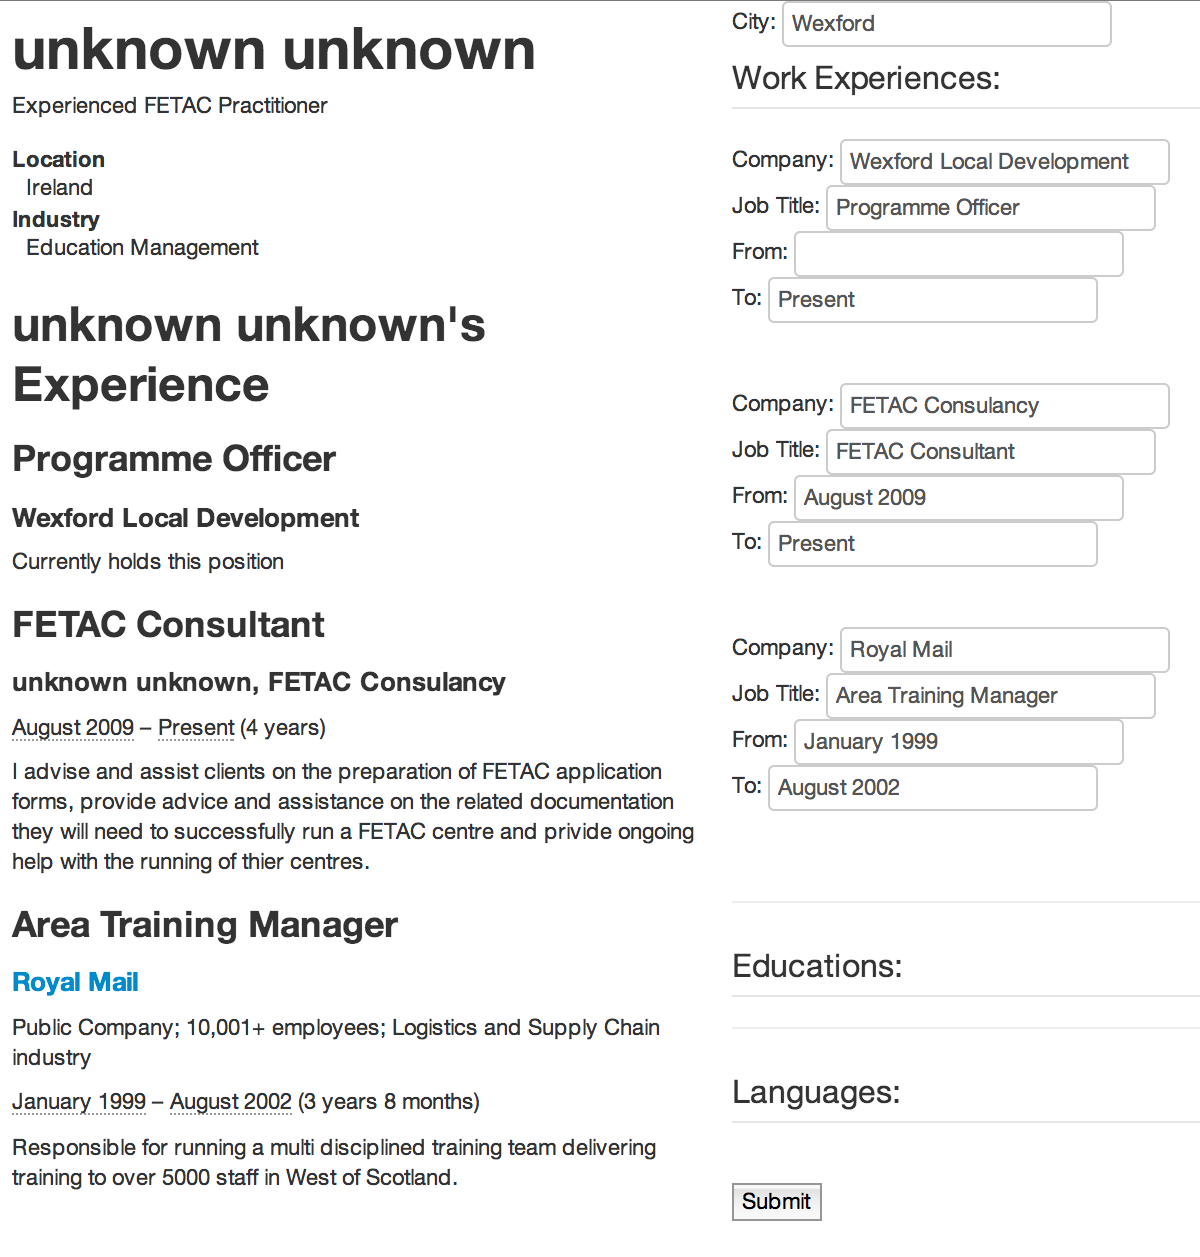
\includegraphics[width=1.0\textwidth]{images/user-input.png}
	\caption{Online user evaluation website: User manually extracted data\protect}
	\label{fig:UserInput}
\end{figure}

\subsubsection{Results}

After the user evaluation, we take user input as the ground truth, we use string matching to compare entered data with automatic extracted data. If the string matching return false, we manually examine the data and decide whether the extracted data is correct.

The metrics here we use are precision, recall and f-measure.
\begin{equation}\label{eq:precision}
	precision=\frac{correctly\_predicted}{predicted}
\end{equation}
\begin{equation}\label{eq:recall}
	recall=\frac{correctly\_predicted}{total}
\end{equation}
\begin{equation}\label{eq:fmeasure}
	f-measure=\frac{2 * precision * recall }{precision + recall}
\end{equation}

The meaning of these metrics can be explained as follows\cite{powers2011evaluation}: Precision, or confidence, is focus on how good we are predicting; Recall, or sensitivity is a measure of the proportion we correctly predicted over total data size. F-measure, or F-score is designed to capture both precision and recall. In order to get high F-score, precision and recall must be high.

\begin{table}[H]
	\centering
	\DTLloaddb[keys={user,precision,recall,fmeasure}]{citycsv}{csvs/city.csv}
	\caption{Precision, recall and f-measure scores for city information}
	\begin{tabular}{|c|c|c|c|}
	\toprule \hline 
	\bfseries User & \bfseries Precision & \bfseries Recall & \bfseries F-Measure
	\DTLforeach{citycsv}{\user=user, \precision=precision, \recall=recall, \fmeasure=fmeasure}{%
	\ifthenelse{\value{DTLrowi}=1}{\tabularnewline \hline}{\tabularnewline \hline}
	\user & \round{\precision} & \round{\recall} & \round{\fmeasure} } \\
	\hline \bottomrule
	\end{tabular}
	\label{tab:cityResult}
\end{table}

According to Table~\ref{tab:cityResult}, users are quite satisfy with our city information extraction strategy. Even some lazy volunteers didn't fill in the ground truth, we still getting average of 0.85 F-score. It's acceptable for us to do complex query using person's city information.

\begin{table}[H]
	\centering
	\DTLloaddb[keys={user,precision,recall,fmeasure}]{companycsv}{csvs/company.csv}
	\caption{Precision, recall and f-measure scores for company information}
	\begin{tabular}{|c|c|c|c|}
	\toprule \hline 
	\bfseries User & \bfseries Precision & \bfseries Recall & \bfseries F-Measure
	\DTLforeach{companycsv}{\user=user, \precision=precision, \recall=recall, \fmeasure=fmeasure}{%
	\ifthenelse{\value{DTLrowi}=1}{\tabularnewline \hline}{\tabularnewline \hline}
	\user & \round{\precision} & \round{\recall} & \round{\fmeasure}} \\
	\hline \bottomrule
	\end{tabular}
	\label{tab:companyResult}
\end{table}

We are getting very high score in company name field according to Table~\ref{tab:companyResult}. The reason for that is because participants normally copy and paste the company name to fill in our survey forms, the exact matching is very high.

\begin{table}[H]
	\centering
	\DTLloaddb[keys={user,precision,recall,fmeasure}]{jobtitlecsv}{csvs/job_title.csv}
	\caption{Precision, recall and f-measure scores for job title information}
	\begin{tabular}{|c|c|c|c|}
	\toprule \hline 
	\bfseries User & \bfseries Precision & \bfseries Recall & \bfseries F-Measure
	\DTLforeach{jobtitlecsv}{\user=user, \precision=precision, \recall=recall, \fmeasure=fmeasure}{%
	\ifthenelse{\value{DTLrowi}=1}{\tabularnewline \hline}{\tabularnewline \hline}
	\user & \round{\precision} & \round{\recall} & \round{\fmeasure}} \\
	\hline \bottomrule
	\end{tabular}
	\label{tab:jobtitleResult}
\end{table}

For the job title field in Table~\ref{tab:jobtitleResult}, the result is similar to the company name field. Users normally copy and paste the text without any term generalisation (e.g. change product manager to manager as it's more general), that's what our parser do as well. So the score is very high.

\begin{table}[H]
	\centering
	\DTLloaddb[keys={user,precision,recall,fmeasure}]{experiencefromcsv}{csvs/experience_from.csv}
	\caption{Precision, recall and f-measure scores for experience start date information}
	\begin{tabular}{|c|c|c|c|}
	\toprule \hline 
	\bfseries User & \bfseries Precision & \bfseries Recall & \bfseries F-Measure
	\DTLforeach{experiencefromcsv}{\user=user, \precision=precision, \recall=recall, \fmeasure=fmeasure}{%
	\ifthenelse{\value{DTLrowi}=1}{\tabularnewline \hline}{\tabularnewline \hline}
	\user & \round{\precision} & \round{\recall} & \round{\fmeasure}} \\
	\hline \bottomrule
	\end{tabular}
	\label{tab:experiencefromResult}
\end{table}

\begin{table}[H]
	\centering
	\DTLloaddb[keys={user,precision,recall,fmeasure}]{experiencetocsv}{csvs/experience_to.csv}
	\caption{Precision, recall and f-measure scores for experience end date information}
	\begin{tabular}{|c|c|c|c|}
	\toprule \hline 
	\bfseries User & \bfseries Precision & \bfseries Recall & \bfseries F-Measure
	\DTLforeach{experiencetocsv}{\user=user, \precision=precision, \recall=recall, \fmeasure=fmeasure}{%
	\ifthenelse{\value{DTLrowi}=1}{\tabularnewline \hline}{\tabularnewline \hline}
	\user & \round{\precision} & \round{\recall} & \round{\fmeasure}} \\
	\hline \bottomrule
	\end{tabular}
	\label{tab:experiencetoResult}
\end{table}

Table~\ref{tab:experiencefromResult} and Table~\ref{tab:experiencetoResult} illustrate our prediction on start date and end date. The precision is high is because LinkedIn always use same datetime pattern to represent the start date and end date. The recall is low is because some profiles do not have the these fields.

The previous four tables (Table~\ref{tab:companyResult}, Table~\ref{tab:jobtitleResult}, Table~\ref{tab:experiencefromResult} and Table~\ref{tab:experiencetoResult}) illustrate our parsed result for work experiences (company name, job title, job start date and job end date). With the average F-score greater than 0.9, we can accept the parse result. The reason for such high result in both company name and job title is, we didn't perform data normalisation in these two fields. Basically, volunteers copy and paste these information to our survey form, and that's what our parser do as well. Since strings are fully matched, the scores are high.

\begin{table}[H]
	\centering
	\DTLloaddb[keys={user,precision,recall,fmeasure}]{collegecsv}{csvs/college.csv}
	\caption{Precision, recall and f-measure scores for college information}
	\begin{tabular}{|c|c|c|c|}
	\toprule \hline 
	\bfseries User & \bfseries Precision & \bfseries Recall & \bfseries F-Measure
	\DTLforeach{collegecsv}{\user=user, \precision=precision, \recall=recall, \fmeasure=fmeasure}{%
	\ifthenelse{\value{DTLrowi}=1}{\tabularnewline \hline}{\tabularnewline \hline}
	\user & \round{\precision} & \round{\recall} & \round{\fmeasure}} \\
	\hline \bottomrule
	\end{tabular}
	\label{tab:collegeResult}
\end{table}

We are getting high score for college name field(Table~\ref{tab:collegeResult}, the explaination for high score is the same as company name field, users just copy and paste the college name from the profile. However, one difference is that we also use our data normalisation tool to classify college name to our ground truth college name. Because in our implementation of college name normalisation, if we couln't find any similar string, we create a new entry in our search engine database and assume it's a new college name.

\begin{table}[H]
	\centering
	\DTLloaddb[keys={user,precision,recall,fmeasure}]{majorcsv}{csvs/major.csv}
	\caption{Precision, recall and f-measure scores for major information}
	\begin{tabular}{|c|c|c|c|}
	\toprule \hline 
	\bfseries User & \bfseries Precision & \bfseries Recall & \bfseries F-Measure
	\DTLforeach{majorcsv}{\user=user, \precision=precision, \recall=recall, \fmeasure=fmeasure}{%
	\ifthenelse{\value{DTLrowi}=1}{\tabularnewline \hline}{\tabularnewline \hline}
	\user & \round{\precision} & \round{\recall} & \round{\fmeasure}} \\
	\hline \bottomrule
	\end{tabular}
	\label{tab:majorResult}
\end{table}

According to Table~\ref{tab:majorResult}, our scores for major field are very low. If we look at the low scores and high scores carefully, we can see that they come in a pair. That means the user input data is consistent, and in some groups of profiles, our data normalisation fail to normalise degree information correctly. The reason for that is people do some data cleaning in their minds so the major information they fill in is cleaned and well known. But our system didn't do any language processing, so the result of a simple copy and paste approach is different from the result generated by human mind.

\begin{table}[H]
	\centering
	\DTLloaddb[keys={user,precision,recall,fmeasure}]{degreecsv}{csvs/degree.csv}
	\caption{Precision, recall and f-measure scores for degree information}
	\begin{tabular}{|c|c|c|c|}
	\toprule \hline 
	\bfseries User & \bfseries Precision & \bfseries Recall & \bfseries F-Measure
	\DTLforeach{degreecsv}{\user=user, \precision=precision, \recall=recall, \fmeasure=fmeasure}{%
	\ifthenelse{\value{DTLrowi}=1}{\tabularnewline \hline}{\tabularnewline \hline}
	\user & \round{\precision} & \round{\recall} & \round{\fmeasure}} \\
	\hline \bottomrule
	\end{tabular}
	\label{tab:degreeResult}
\end{table}

We are getting very high degree score in Table~\ref{tab:degreeResult}, which means our ground truth degrees in working properly and classified most of the degree information correctly.

\begin{table}[H]
	\centering
	\DTLloaddb[keys={user,precision,recall,fmeasure}]{educationfromcsv}{csvs/education_from.csv}
	\caption{Precision, recall and f-measure scores for education start date information}
	\begin{tabular}{|c|c|c|c|}
	\toprule \hline 
	\bfseries User & \bfseries Precision & \bfseries Recall & \bfseries F-Measure
	\DTLforeach{educationfromcsv}{\user=user, \precision=precision, \recall=recall, \fmeasure=fmeasure}{%
	\ifthenelse{\value{DTLrowi}=1}{\tabularnewline \hline}{\tabularnewline \hline}
	\user & \round{\precision} & \round{\recall} & \round{\fmeasure}} \\
	\hline \bottomrule
	\end{tabular}
	\label{tab:educationfromResult}
\end{table}

\begin{table}[H]
	\centering
	\DTLloaddb[keys={user,precision,recall,fmeasure}]{educationtocsv}{csvs/education_to.csv}
	\caption{Precision, recall and f-measure scores for education end date information}
	\begin{tabular}{|c|c|c|c|}
	\toprule \hline 
	\bfseries User & \bfseries Precision & \bfseries Recall & \bfseries F-Measure
	\DTLforeach{educationtocsv}{\user=user, \precision=precision, \recall=recall, \fmeasure=fmeasure}{%
	\ifthenelse{\value{DTLrowi}=1}{\tabularnewline \hline}{\tabularnewline \hline}
	\user & \round{\precision} & \round{\recall} & \round{\fmeasure}} \\
	\hline \bottomrule
	\end{tabular}
	\label{tab:educationtoResult}
\end{table}

The scores for college start date (Table~\ref{tab:educationfromResult}) and college end date (Table~\ref{tab:educationtoResult}) didn't perform well. This evaluation helps us discover a problem in extracting these two fields. Since our system makes a wrong assumption about the format of the start date and end date(as 'yyyy-mm-dd'), we could not capture the fact that the start date and end date format in education background is 'yyyy'. This finding also prove that doing user study is very important in system evaluation.

\begin{figure}[H]
	\centering
	\includegraphics[width=1.0\textwidth]{images/evaluation/summary_scores.png}
	\caption{Summary: average precion, recall, f-measure for all fields}
	\label{fig:summaryPRF}
\end{figure}

From Figure~\ref{fig:summaryPRF}, we can see that city, company names, job titles, work experience start and end date, college names and degree information have high average scores. But for major, we got an average f-score a bit greate than 0.6, which means we cannot correctly classify the major names. In the future, we might need natural language processing and college subjects database to get a better results. And we need to fix the problem in extracting college start date and college end date.

\subsection{User perceived data quality}
Apart from precisions, recalls and F-measure, we also collect user ratings for each field and user overall rating for each profile. Figure~\ref{fig:UserCompare} is the screenshot that asking user to compare their manually extracted data with our automatically extracted data and rating our results.

\begin{figure}[H]
	\centering
	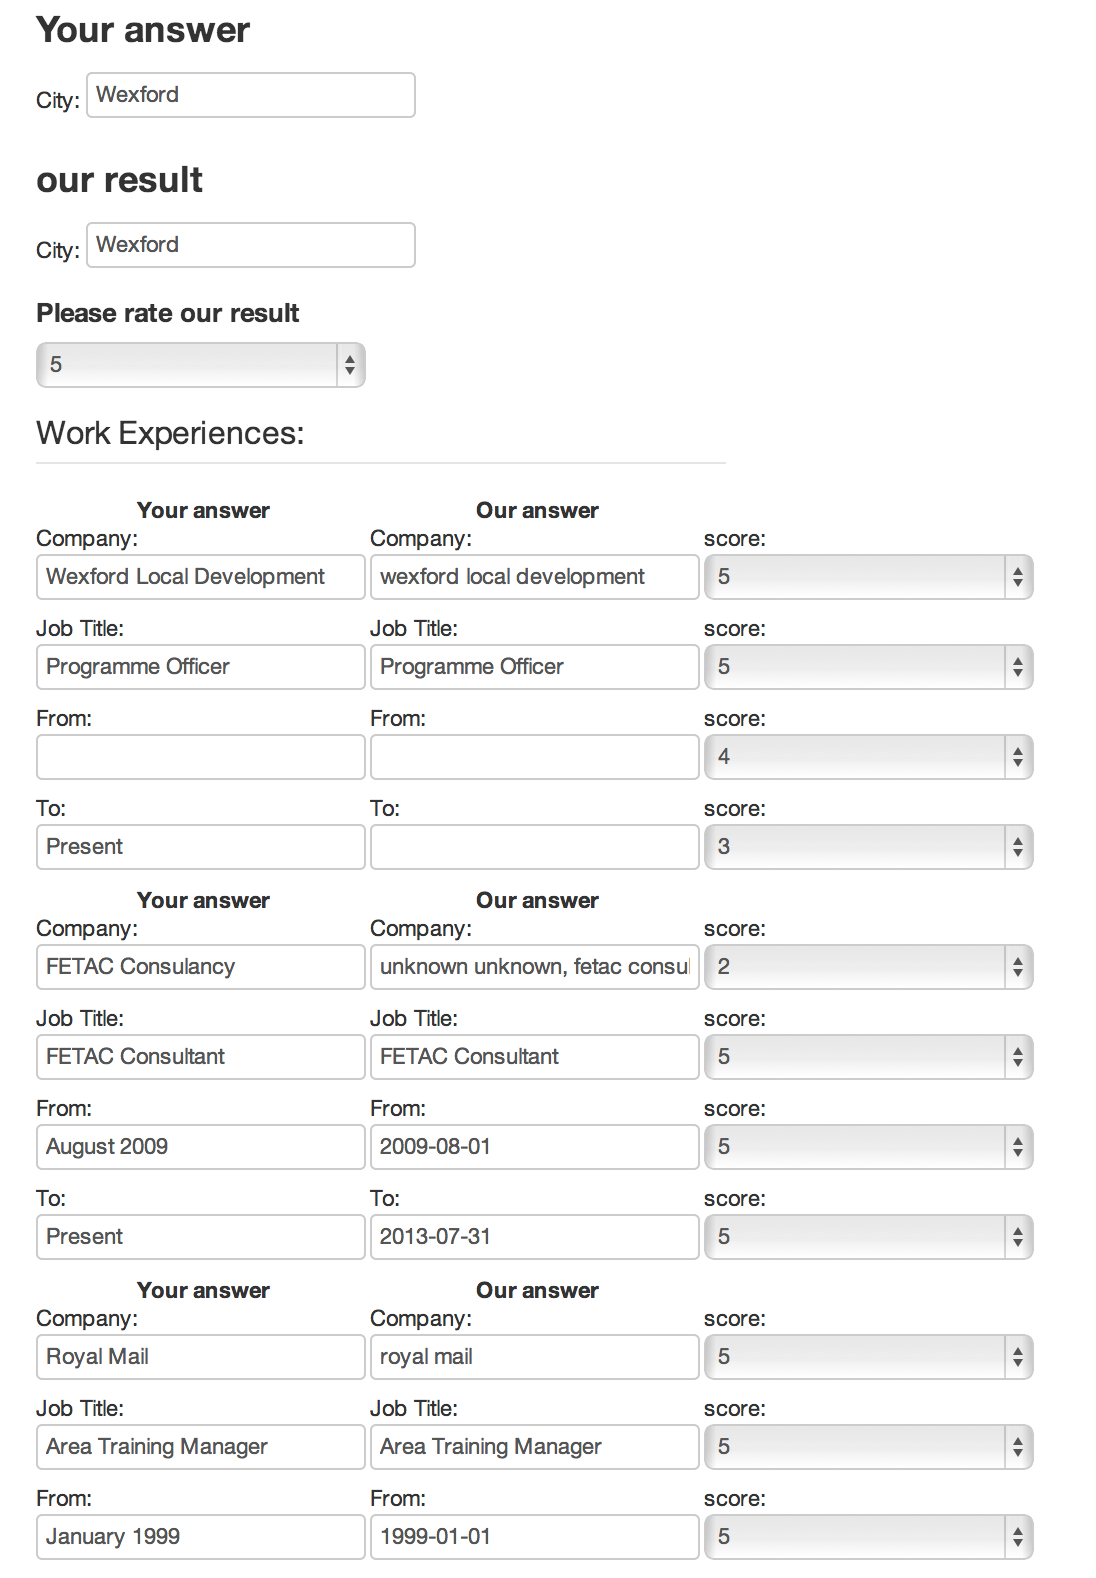
\includegraphics[scale=0.8]{images/user-compare.png}
	\caption{Online user evaluation website: Asking user compare manually extracted data with automatically extracted data\protect}
	\label{fig:UserCompare}
\end{figure}

At here we only show average rating for each field. From these ratings, we want to get consistent results about how well is our parser and data normalisation working as in \nameref{subsec:accuracy}. 

\begin{figure}[H]
\centering
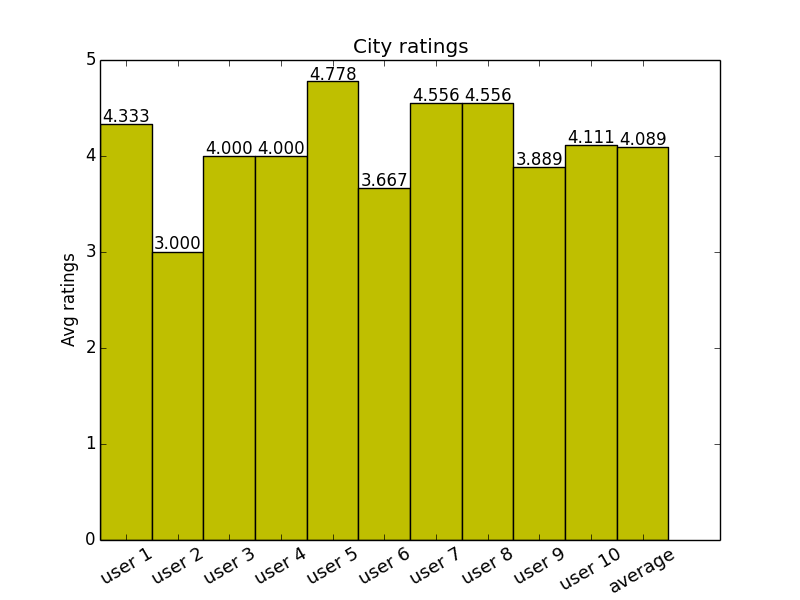
\includegraphics[width=110mm]{images/evaluation/average_city_score.png}
\caption{User average rating for city}
\label{fig:city}
\end{figure}

In Figure~\ref{fig:city} we find the user satisfaction ratings are not fully match with Table\ref{tab:cityResult}. The reason for that is our city extraction strategy is setting the first return possible city from all cities as the person's current living city. Since the profile sometime contains too less information for us to guess where the person is actually located, some users simply don't like our result when they see ``A person work for Tesco Ireland is now living in Limerick'' as they think there's too few information to predict the correct city.

\begin{figure}[H]
\centering
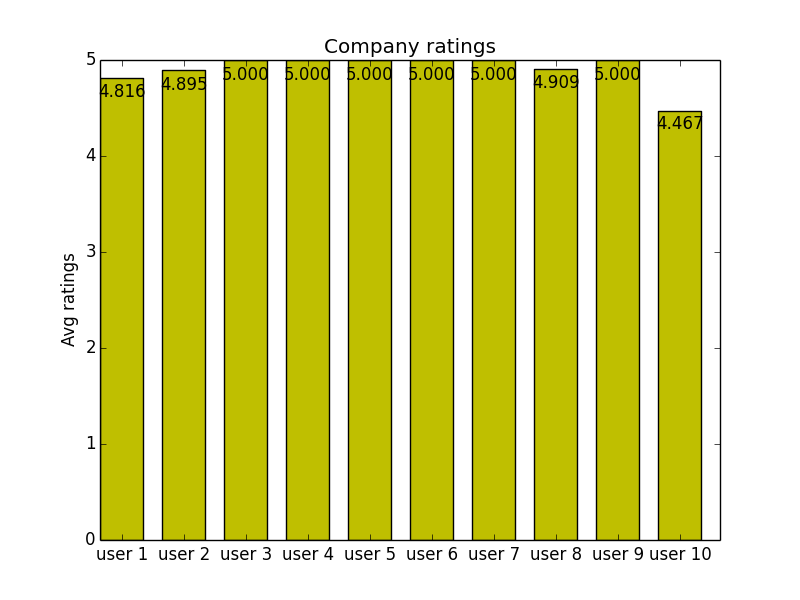
\includegraphics[width=110mm]{images/evaluation/average_company_score.png}
\caption{User average rating for company name}
\label{fig:company}
\end{figure}

\begin{figure}[H]
\centering
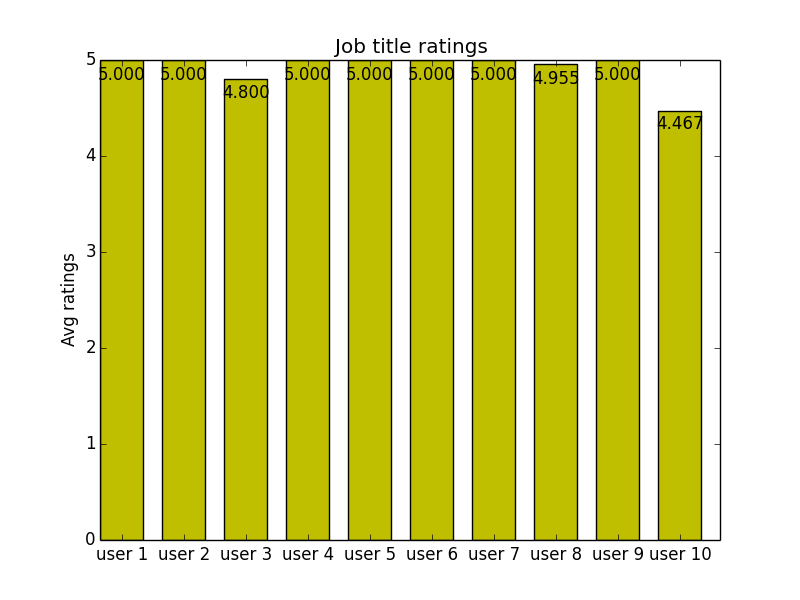
\includegraphics[width=110mm]{images/evaluation/average_job_title_score.png}
\caption{User average rating for job title}
\label{fig:job_title}
\end{figure}

In Figure~\ref{fig:company} and Figure~\ref{fig:job_title}, We get consistent result with Table~\ref{tab:companyResult} and Table~\ref{tab:jobtitleResult}. As we discussed earlier, a simple copy and paste approach is accepted by our participants.

\begin{figure}[H]
\centering
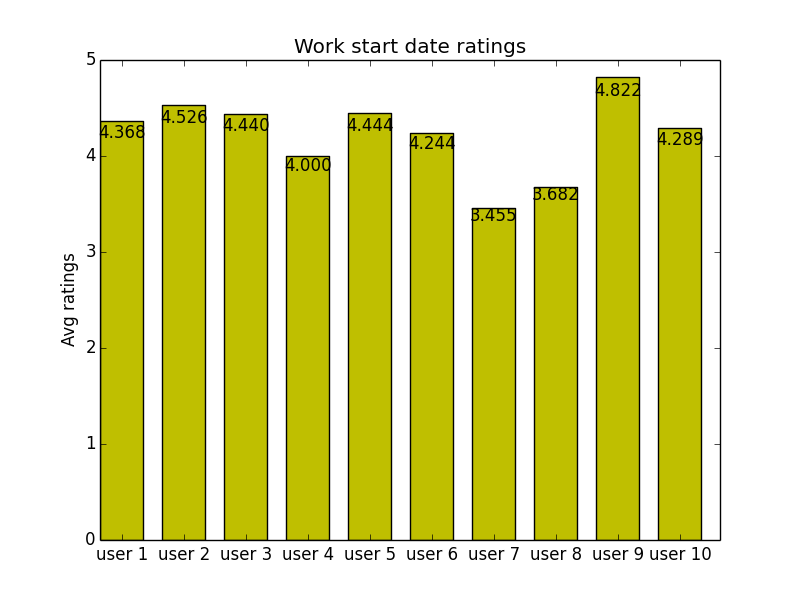
\includegraphics[width=110mm]{images/evaluation/average_experience_start_date_score.png}
\caption{User average rating for experience start date}
\label{fig:experiencestart}
\end{figure}

\begin{figure}[H]
\centering
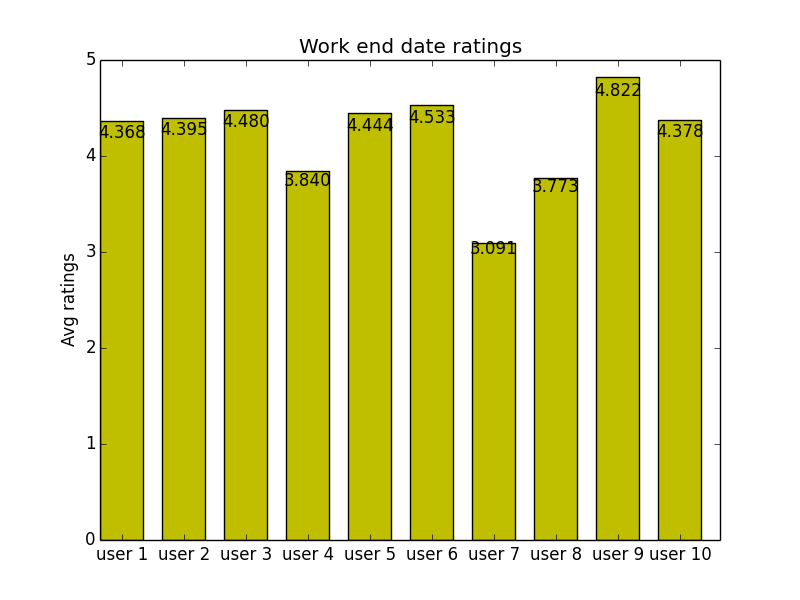
\includegraphics[width=110mm]{images/evaluation/average_experience_end_date_score.png}
\caption{User average rating for experience end date}
\label{fig:experienceend}
\end{figure}

For the start date ratings (Figure~\ref{fig:experiencestart}) and end date ratings (Figure~\ref{fig:experienceend}), we are getting lower user satisfaction comparing to what we get at the previous section (Table~\ref{tab:experiencefromResult} and Table~\ref{tab:experiencetoResult}). The reason for that is, some volunteers do not happy we convert the datetime format from 'MM yyyy' to 'yyyy-mm-01'. What we are doing here is we assume all the start date and end date of a work experience is on the first day of the month. We explain the reason to volunteers during the evaluation, as we need this format the match the date literal definition in XML Schema\cite{biron2004xml}.

\begin{figure}[H]
\centering
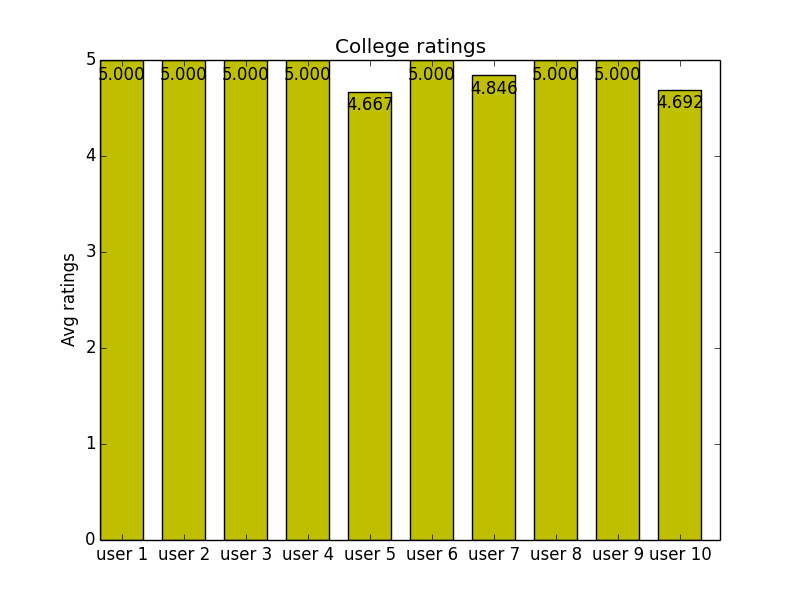
\includegraphics[width=110mm]{images/evaluation/average_college_score.png}
\caption{User average rating for college}
\label{fig:college}
\end{figure}

Similar to Figure~\ref{fig:company}, our user average rating for college names (Figure~\ref{fig:college}) is widely accepted. Even we try to use our data normalisation module to classify the college name, but when we encounter a new unknown college name, we add it to our Lucene text search engine database instead of leaving the college name empty.

\begin{figure}[H]
\centering
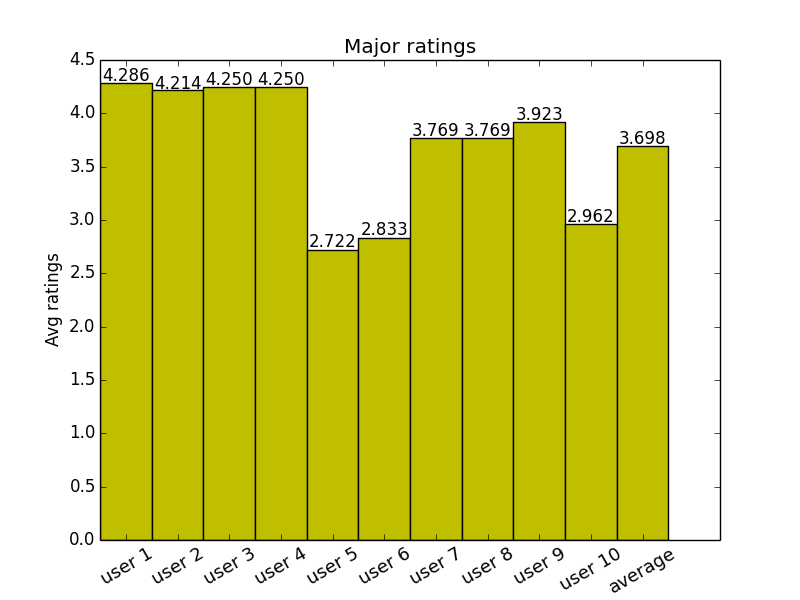
\includegraphics[width=110mm]{images/evaluation/average_major_score.png}
\caption{User average rating for major}
\label{fig:major}
\end{figure}

Because every two users are viewing same 10 randomly selected profiles, therefore, for major field, the average ratings (Figure~\ref{fig:major}) from user 5 and user 6 are so low is because our parser perform bad in that 10 profiles. Notice that the user ratings for major field is actually higher than the scores we get in Table\ref{tab:majorResult}, that is because participants are happy to know that our system is not that intelligent as human mind and fail to clean the major field correctly. So participants rate their satisfaction scores high.

\begin{figure}[H]
\centering
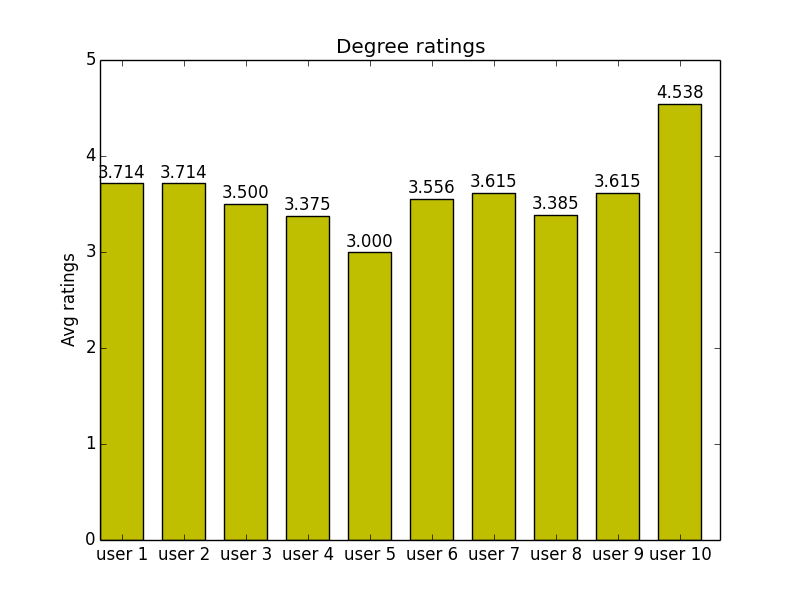
\includegraphics[width=110mm]{images/evaluation/average_degree_score.png}
\caption{User average rating for degree}
\label{fig:degree}
\end{figure}

We are getting lower user ratings at degree fields (Figure~\ref{fig:degree}) comparing to \autoref{tab:degreeResult}. That's because the data completeness for degree field is low. For every profile that has no degree field, we set the score to 3, which is the average score by default.

\begin{figure}[H]
\centering
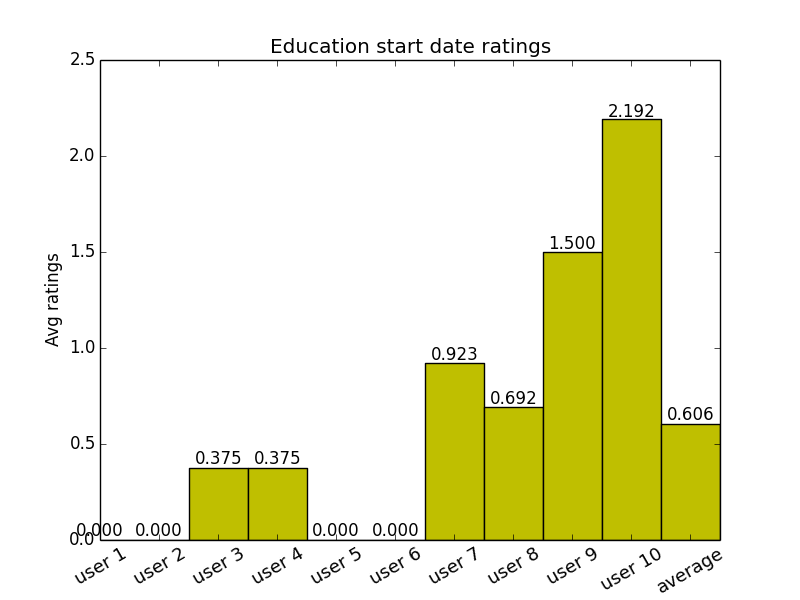
\includegraphics[width=110mm]{images/evaluation/average_education_start_date_score.png}
\caption{User average rating for education start date}
\label{fig:educationstart}
\end{figure}

\begin{figure}[H]
\centering
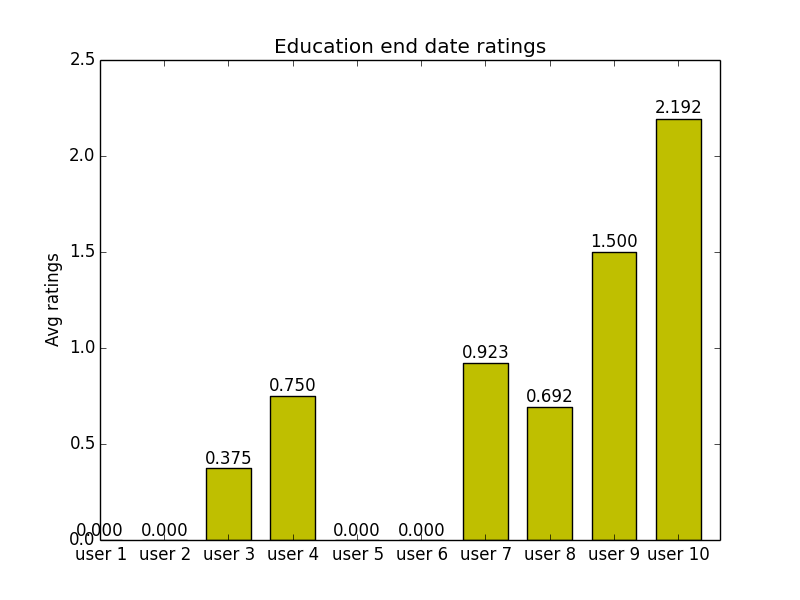
\includegraphics[width=110mm]{images/evaluation/average_education_end_date_score.png}
\caption{User average rating for education end date}
\label{fig:educationend}
\end{figure}

As mentioned in the previous section, our parser failed to capture the fact that education start date and education end date is using 'yyyy' pattern in representing the datetime. Therefore, most of our volunteers just set the rating to 0 since thre's no information available (Figure~\ref{fig:educationstart} and Figure~\ref{fig:educationend}).

\begin{figure}
	\centering
	\includegraphics[width=1.0\textwidth]{images/evaluation/summary_ratings.png}
	\caption{Summary: average user ratings for all fields}
	\label{fig:SummaryRatings}
\end{figure}

Figure~\ref{fig:SummaryRatings} shows average user ratings for all fields. As we can see, users are quite satisfy with our results in city, company name, job title, work experience start date and end date. And users are slightly not happy with our result in major and degree, which is what we need to improve in the future. Finally users are totally not accept the empty college start date and end date.

\subsection{Metadata fitness}

This section is a reflection on how the extracted triples fit to the data visualisation interface. The interface is divided into 3 scenarios: 

\begin{description}
	\item Scenario 1, Government \hfill \\
	The first scenario is that the interface should reflect the needs of Government officers. The fields that used by them are: city, industry type, academic degree and company size.
	\item Scenario 2, Company's human resource department \hfill \\
	The user interface also support daily queries from HR. The fields that used in this scenario are: city, degree, skill, work experience and start date.
	\item Scenario 3, Job seekers and college students
	This part allows users get insights about the employment status by city. The fields that used in this scenario are: city, degree, skill and position.
\end{description}

During the development and evaluation, we found there're some drawbacks of the extracted data that makes the query and the user interface hard to develop and use:
\begin{enumerate}
	\item Do not have information to group similar job title together. This is important as we want our query return more correct result and in the meantime keeps the query as simple as possible. For example, when one querying ``software engineer'' similar terms such as ``application developer, Java software engineer'' should all return as these job titles have no significant difference if we want to compare this job in IT over another industry. Doing this classification is hard, we will discuss it in future work section in the next chapter.
	\item Company names may have aliases. One example is ``Oracle'' and ``Oracle EMEA''. But since we cannot find company names database as ground truth, our system cannot handle this problem. This issue is very similar to the previous one, it needs we have very accurate ground truth.
	\item As SPARQL has very limit function in datetime manipulation, the start date and end date approach in our model is not working really well. For example, if one user is looking for ``How many people had been working in a company for more then 5 years?''. The query is very hard to write so it would be easier if our model have ``year between'' field that address this requirement.
\end{enumerate}

The details of possible solution of drawbacks will be discussed in next chapter, future works section.

\section{System performance}

In \nameref{subsec:env}, we list our software and hardware details. Here we want to show the performance of some critical modules, to provide more comprehensive details of the system. One important things to know is that the performance measurements does not include database accessing and file serialisation and other miscellaneous, therefore, in production environment, the system performance could be less than the result we got.

\subsection{Parsing performance}
We run our parser 10 times, each time it parses 100 randomly selected profiles, the average time spending on parsing 100 profiles is: 18.27 seconds.

\subsection{Normalising and converting performance}
We run our RDF converter 10 times, each time in try to normalise the data in 100 profiles and convert it into RDF triples, the average time spending on this is: 345.53 seconds.

\newacronym{io}{IO}{input \& output}
\subsection{Query performance}
We tried several queries with different level of complexity. Because some simple queries (for example, returning all triples) are simple but it takes a very long time on File \acrshort{io}, so we manually set ``soft limit'' equals to 2000 for all queries. The ``soft limit'' means the maximum number of rows returned is 2000. Below is server case and the corresponding time:

\subsubsection{Simple query that only return subject, predicate and object}

\begin{Verbatim}[frame=single]
	select * where {?subject ?predicate ?object. }
\end{Verbatim}

The time spend on this query is: 0.548360s, and it returned 2000 rows.

\subsubsection{Simple query that asks from subject, predicate and object then summing up the subject}
\begin{Verbatim}[frame=single]
	select (count(?subject) as ?total) where  {
		?subject ?predicate ?object. 
	}
\end{Verbatim}
The time spend on this query is: 0.021132s, and it returned 1 rows.
Notice that this query is 27 times faster that the previous query even though the complexity is higher. We don't know the implementation of 4store, but one possible explaination is that the COUNT method can be optimised so the program do not really need read 2000 rows to get the actually result.

\subsubsection{A query that defines two relationships}
\begin{Verbatim}[frame=single]
	select * where {
		?person a foaf:Person;
			lk:skill ?skill.
	}
\end{Verbatim}
The time spend on this query is: 0.134334s, and it returned 2000 rows.
It is an interesting result because getting graph patterns is actually quicker than the first query, which only ask for all triples. One possible answer is the 4store SPARQL engine has special optimisation on graph matching.

\subsubsection{A query that defines two relationships with group by and count}
\begin{Verbatim}[frame=single]
	select ?city (count(?person) as ?pCount) where {
		?person a foaf:Person ;
			dbpedia-owl:city ?city .
	} group by ?city
\end{Verbatim}
The time spend on this query is: 0.011658s, and it returned 18 rows.
This time, data aggregation query is actually quicker than simple ``print all'' query. This result demonstrate 4store implementation of data aggregation has very high performance.

\subsubsection{A query that defines two relationships with group by, count and order by}
\begin{Verbatim}[frame=single]
	select ?skill (count(?skill) as ?sCount) where{
		?p a foaf:Person;
			lk:skill ?skill.
	} group by ?skill order by desc(?sCount)
\end{Verbatim}
The time spend on this query is: 7.770524s, and it returned 16184 rows.
This query takes very long time to execute. That is because to generate the correct result, the SPARQL engine has to split all the skill into groups and sum them up, there's no optimisation even we specify soft limit equals to 2000.

\subsubsection{Conclusion}
We can see that for complex group by, count and order by query, our system takes too long time to respond. One important factor that result in slow queries is the system hardware. Because we test the performance in production environment, the machine is an Amazon EC2 m1.medium instance. The hardware parameters are listed at \autoref{subsec:env}, which is relatively low comparing to current standard server. Therefore, the performance issue can be potentially alleviated by upgrading to a higher \acrlong{cpu}.

\section{Summary}
In this section, we evaluate our result set and SPARQL server thoroughly. We find the fields that are converted with high accuracy and also identify issues that need to be fixed or improved. We examine the performance of our production server and make suggestions for future improvement.
